\documentclass{ximera}

\title{What is Ximera?}

\outcome{Understand what Ximera is and how it can be used}

\begin{document}
\begin{abstract}
An introduction to the Ximera system.
\end{abstract}
\maketitle

\link[Ximera]{http://ximera.osu.edu} is an NSF-funded (DUE-1245433)
open-source software project created at The Ohio State
University. This project facilitates the creation of learning
materials in the form of interactive web pages and high quality PDF
documents.

An author writes content as a \LaTeX\ document.  Ximera uses this
document to produce a both a PDF handout and an interactive online
textbook.

\begin{image}
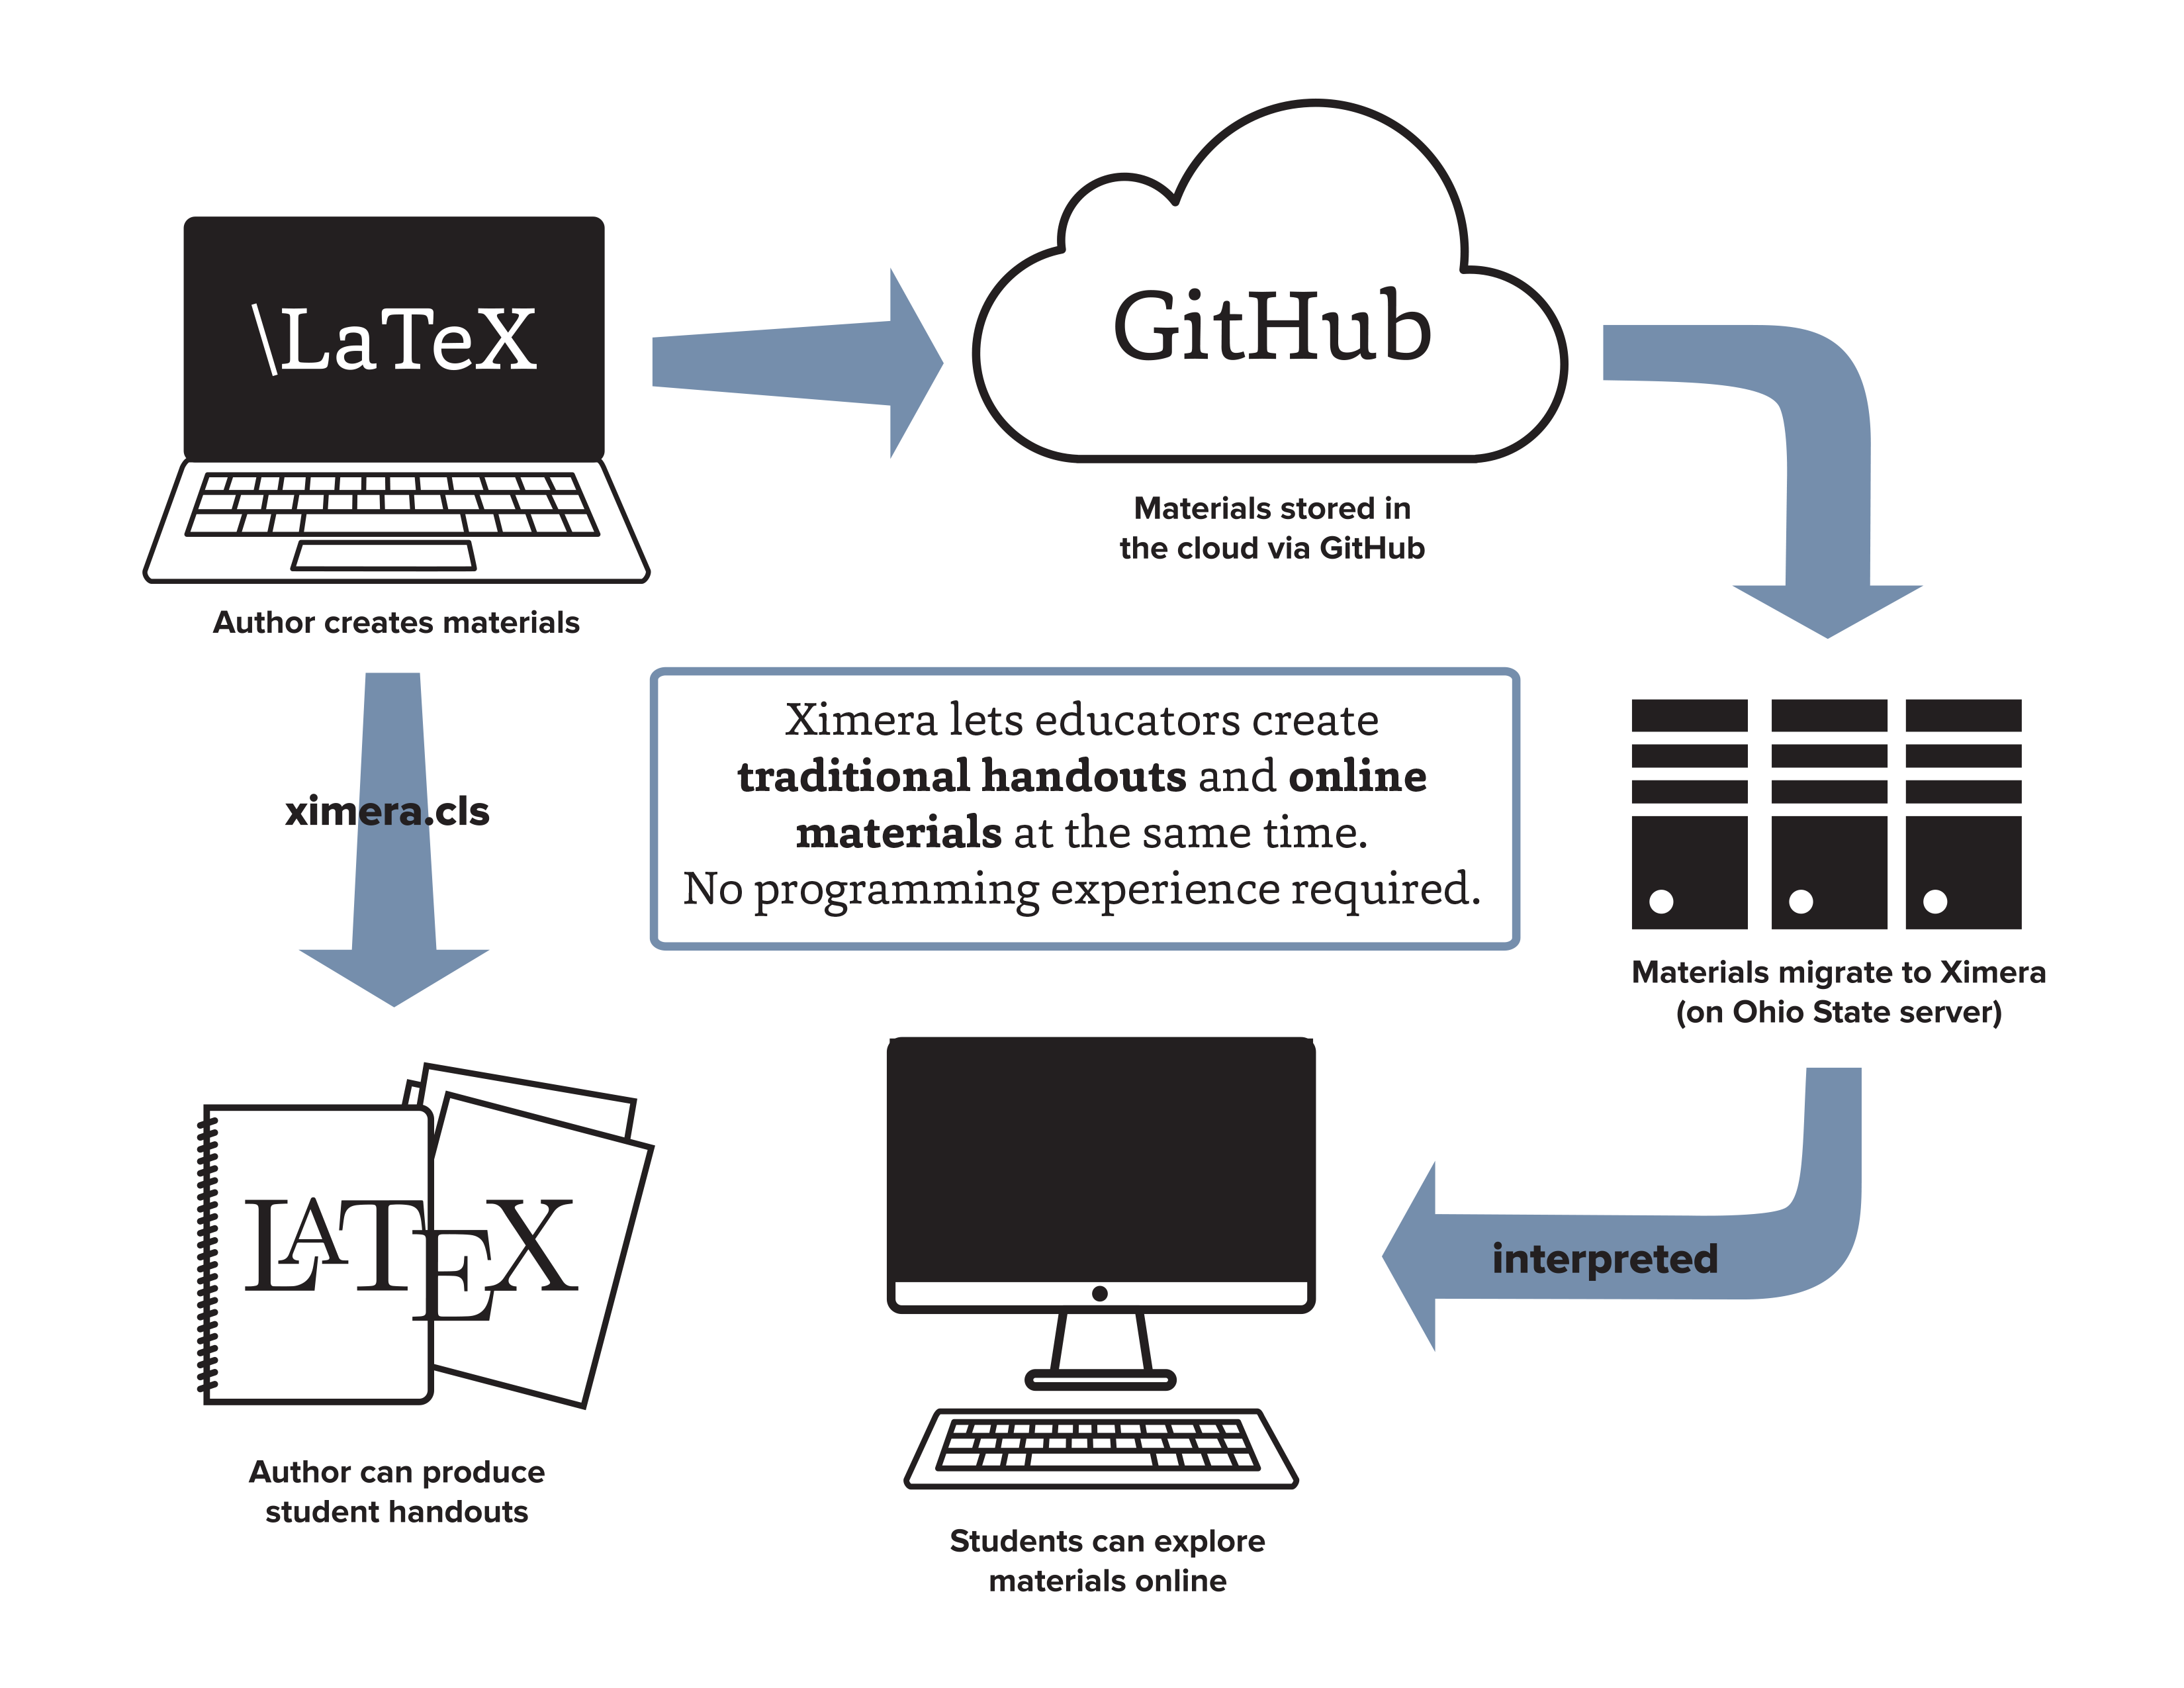
\includegraphics[scale=.25]{./XimeraGraphic.png}
\end{image}

%% For an example activity, see \link[here]{https://ximera.osu.edu/course/mooculus/calculus1/master/definitionOfTheDerivative/digInTheDerivativeViaLimits}

Example courses can be found at the links below:

\begin{itemize}
\item \link[Calculus 1]{http://ximera.osu.edu/course/mooculus/calculus1}
\item \link[Calculus 2]{http://ximera.osu.edu/course/mooculus/calculus2}
\item \link[Calculus $e$]{http://ximera.osu.edu/course/mooculus/calculusE}
\item \link[Calculus 3]{http://ximera.osu.edu/course/mooculus/calculus3}
\item \link[Linear Algebra]{http://ximera.osu.edu/course/mooculus/linearAlgebra}
\end{itemize}

\newpage

%\paragraph{Ximera and solutions}

Ximera addresses and solves many of the problems with commercial
solutions.

\subparagraph{Annual crashes and bugs}

Ximera was initially used in a MOOC setting. In its first deployment,
it was able to handle over $10000$ logins without compromising the
user experience.


\subparagraph{Adhering to other's content}

Books written in Ximera are authored in \LaTeX, the standard for
academic mathematical writing. This will allow faculty at OSU to
refine current content and develop new content for our
courses. Moreover, Ximera is highly modular. Each section is its own
stand-alone compilable document.

%Instructor and coordinator control over content; ``no one wants to give someone else's speech''

\subparagraph{Alignment of content to assessments}

Since the content can be easily modified, course coordinators can
ensure alignment between content and assessment.


\subparagraph{New editions}

Ximera can be edited on-the-fly without detriment to the students. Our
materials will evolve organically to meet our needs.


%% \subparagraph{Outsourcing assessment}
%% Outsourcing assessment is outsourcing a core competency of the University


\subparagraph{High costs}

Ximera is open-source. It provides a PDF version of the text that can
either be printed out, or sold on a ``publishing on demand'' website
for a minimal cost.


\subparagraph{Longevity}
Ximera is available to all, regardless of whether a student is
enrolled in a course.


%% \subparagraph{Opaqueness}
%% The transparency (or rather opaqueness) of adaptive grading in commercial platforms

\subparagraph{Interaction data is unavailable}

All data concerning student interaction with Ximera is available.



\end{document}
